\chapter{Tab 5 · Graphs}\label{ch:graphs}

\section{How graphs are drawn}
All graphs are SVG drawn by one function, \texttt{svgPlot()}, without any plotting library. The SOP profile supplies the
limits (Cq cut-off, late-signal limit, maximum replicate SD, zone spread), the outcome colours and the labels, so every graph
changes when the profile changes and carries the profile's name, version and SHA-256. Each graph can be saved as SVG or PNG
together with the numbers behind it (CSV); one button saves all graphs of a run and all cross-run graphs as a ZIP.

\par\medskip\noindent{\small\textbf{Listing}~\texttt{svgPlot()}\hfill\textcolor{gray}{HTML lines 4988--5032}}\par\nopagebreak
\lstinputlisting[style=vstyle,language=JavaScript,firstnumber=4988]{code/svgPlot.js}


\par\medskip\noindent{\small\textbf{Listing}~\texttt{niceTicks()}\hfill\textcolor{gray}{HTML lines 4978--4985}}\par\nopagebreak
\lstinputlisting[style=vstyle,language=JavaScript,firstnumber=4978]{code/niceTicks.js}



A graph is one entry of the array \texttt{GRAPHS}: an id, a group, a title, a note and a \texttt{render(c)} function that
returns the SVG and the rows of its CSV.

\par\medskip\noindent{\small\textbf{Listing}~\texttt{GRAPHS entry: amplification curves}\hfill\textcolor{gray}{HTML lines 5079--5097}}\par\nopagebreak
\lstinputlisting[style=vstyle,language=JavaScript,firstnumber=5079]{code/graph_curves.js}


\par\medskip\noindent{\small\textbf{Listing}~\texttt{graphContext()}\hfill\textcolor{gray}{HTML lines 5414--5419}}\par\nopagebreak
\lstinputlisting[style=vstyle,language=JavaScript,firstnumber=5414]{code/graphContext.js}


\par\medskip\noindent{\small\textbf{Listing}~\texttt{graphAllZip()}\hfill\textcolor{gray}{HTML lines 5461--5481}}\par\nopagebreak
\lstinputlisting[style=vstyle,language=JavaScript,firstnumber=5461]{code/graphAllZip.js}



{\footnotesize
\begin{longtable}{@{}llll@{}}
\toprule \textbf{Id} & \textbf{Scope} & \textbf{Title} & \textbf{What it shows} \\\midrule\endfirsthead
\toprule \textbf{Id} & \textbf{Scope} & \textbf{Title} & \textbf{What it shows} \\\midrule\endhead
\texttt{timeline} & run & Run timeline — created, run, an… & Every dated event the file carr… \\\hline
\texttt{curves} & run & Amplification curves coloured b… & Stored curves of the selected t… \\\hline
\texttt{plate} & run & Plate heat map & Every physical position. Choose… \\\hline
\texttt{unanalysed} & run & Signal in wells that are not in… & Rising fluorescence in position… \\\hline
\texttt{cqstrip} & run & Cq by target with SOP cut-offs & One point per well. Colour by S… \\\hline
\texttt{repsd} & run & Replicate spread — mean Cq agai… & One point per sample and target… \\\hline
\texttt{stdcurve} & run & Standard curve with residuals a… & Cq against log10 of the stored … \\\hline
\texttt{ic} & run & Internal control / reference Cq… & Cq of the targets the SOP marks… \\\hline
\texttt{endpoint} & run & Fluorescence level against Cq & End-point fluorescence (or ampl… \\\hline
\texttt{levels} & run & Background and plateau fluoresc… & For each detection channel / ta… \\\hline
\texttt{outcomes} & run & SOP outcomes per target & Number of sample/target results… \\\hline
\texttt{temperature} & run & Block, cover and zone temperatu… & From the instrument log inside … \\\hline
\texttt{recalc} & run & Stored Ct against the Ct re-der… & .eds instrument only: differenc… \\\hline
\texttt{lc\_thermal} & run & Block temperature trace (.ixo i… & The block temperature the .ixo … \\\hline
\texttt{x\_timeline} & all runs & Runs on a calendar — run time a… & Each run as a green dot at its … \\\hline
\texttt{x\_delay} & all runs & Hours from run end to the last … & Processing time per run. The da… \\\hline
\texttt{x\_accept} & all runs & Run acceptance grid & Runs (rows) against the SOP cri… \\\hline
\texttt{x\_outcomes} & all runs & SOP outcomes per run & Stacked counts of sample/target… \\\hline
\texttt{x\_control} & all runs & Control Cq across runs with SOP… & Descriptive control overview. S… \\\hline
\texttt{x\_signal} & all runs & Background and plateau fluoresc… & Median background and median en… \\\hline
\texttt{x\_duration} & all runs & Run duration and instrument use & Minutes from run start to run e… \\\hline
\texttt{x\_findings} & all runs & Forensic findings by area (Pare… & Count of error and review findi… \\\hline
\texttt{x\_control\_batches} & all runs & Control extraction batches & Descriptive association only. S… \\\hline
\texttt{x\_control\_age} & all runs & Control extract age versus Cq & Descriptive association only. S… \\\hline
\texttt{x\_control\_thermal} & all runs & Control Cq versus cooling rate & Descriptive association only. S… \\\hline
\bottomrule
\end{longtable}}



\figui[0.9]{ui_graphs.png}{The Graphs tab: choice of graph and experiment, the graph with the SOP profile it was drawn with, and the download buttons.}{ui_graphs}

\section{Graphs of one run}

\subsection*{Run history}
\fig[0.85]{g_LC_timeline.png}{\texttt{timeline} — every dated event of \texttt{DEMO\_LC1\_SCREEN\_006}: experiment and run created, run started and ended, analyses created and modified, last change.}{g_LC_timeline}

\par\medskip\noindent{\small\textbf{Listing}~\texttt{GRAPHS entry added by the control panel: LightCycler block temperature}\hfill\textcolor{gray}{HTML lines 6810--6815}}\par\nopagebreak
\lstinputlisting[style=vstyle,language=JavaScript,firstnumber=6810]{code/graph_lc_thermal.js}


\fig[0.9]{g_LC_lc_thermal.png}{\texttt{lc\_thermal} — synthetic .ixo instrument block temperature log: 10 min hot start, 45 cycles 95 / 60 / 72\,°C, overshoot at 95\,°C and undershoot at 60\,°C. The display keeps the minimum and maximum of every time slice.}{g_LC_lc_thermal}
\fig[0.9]{g_QS_temperature.png}{\texttt{temperature} — synthetic .eds instrument log: modelled sample temperature, heated cover and the spread of the six block zones ($\times10$) against the SOP limit.}{g_QS_temperature}

\subsection*{Fluorescence}
\begin{figure}[htbp]\centering
\begin{subfigure}{0.49\linewidth}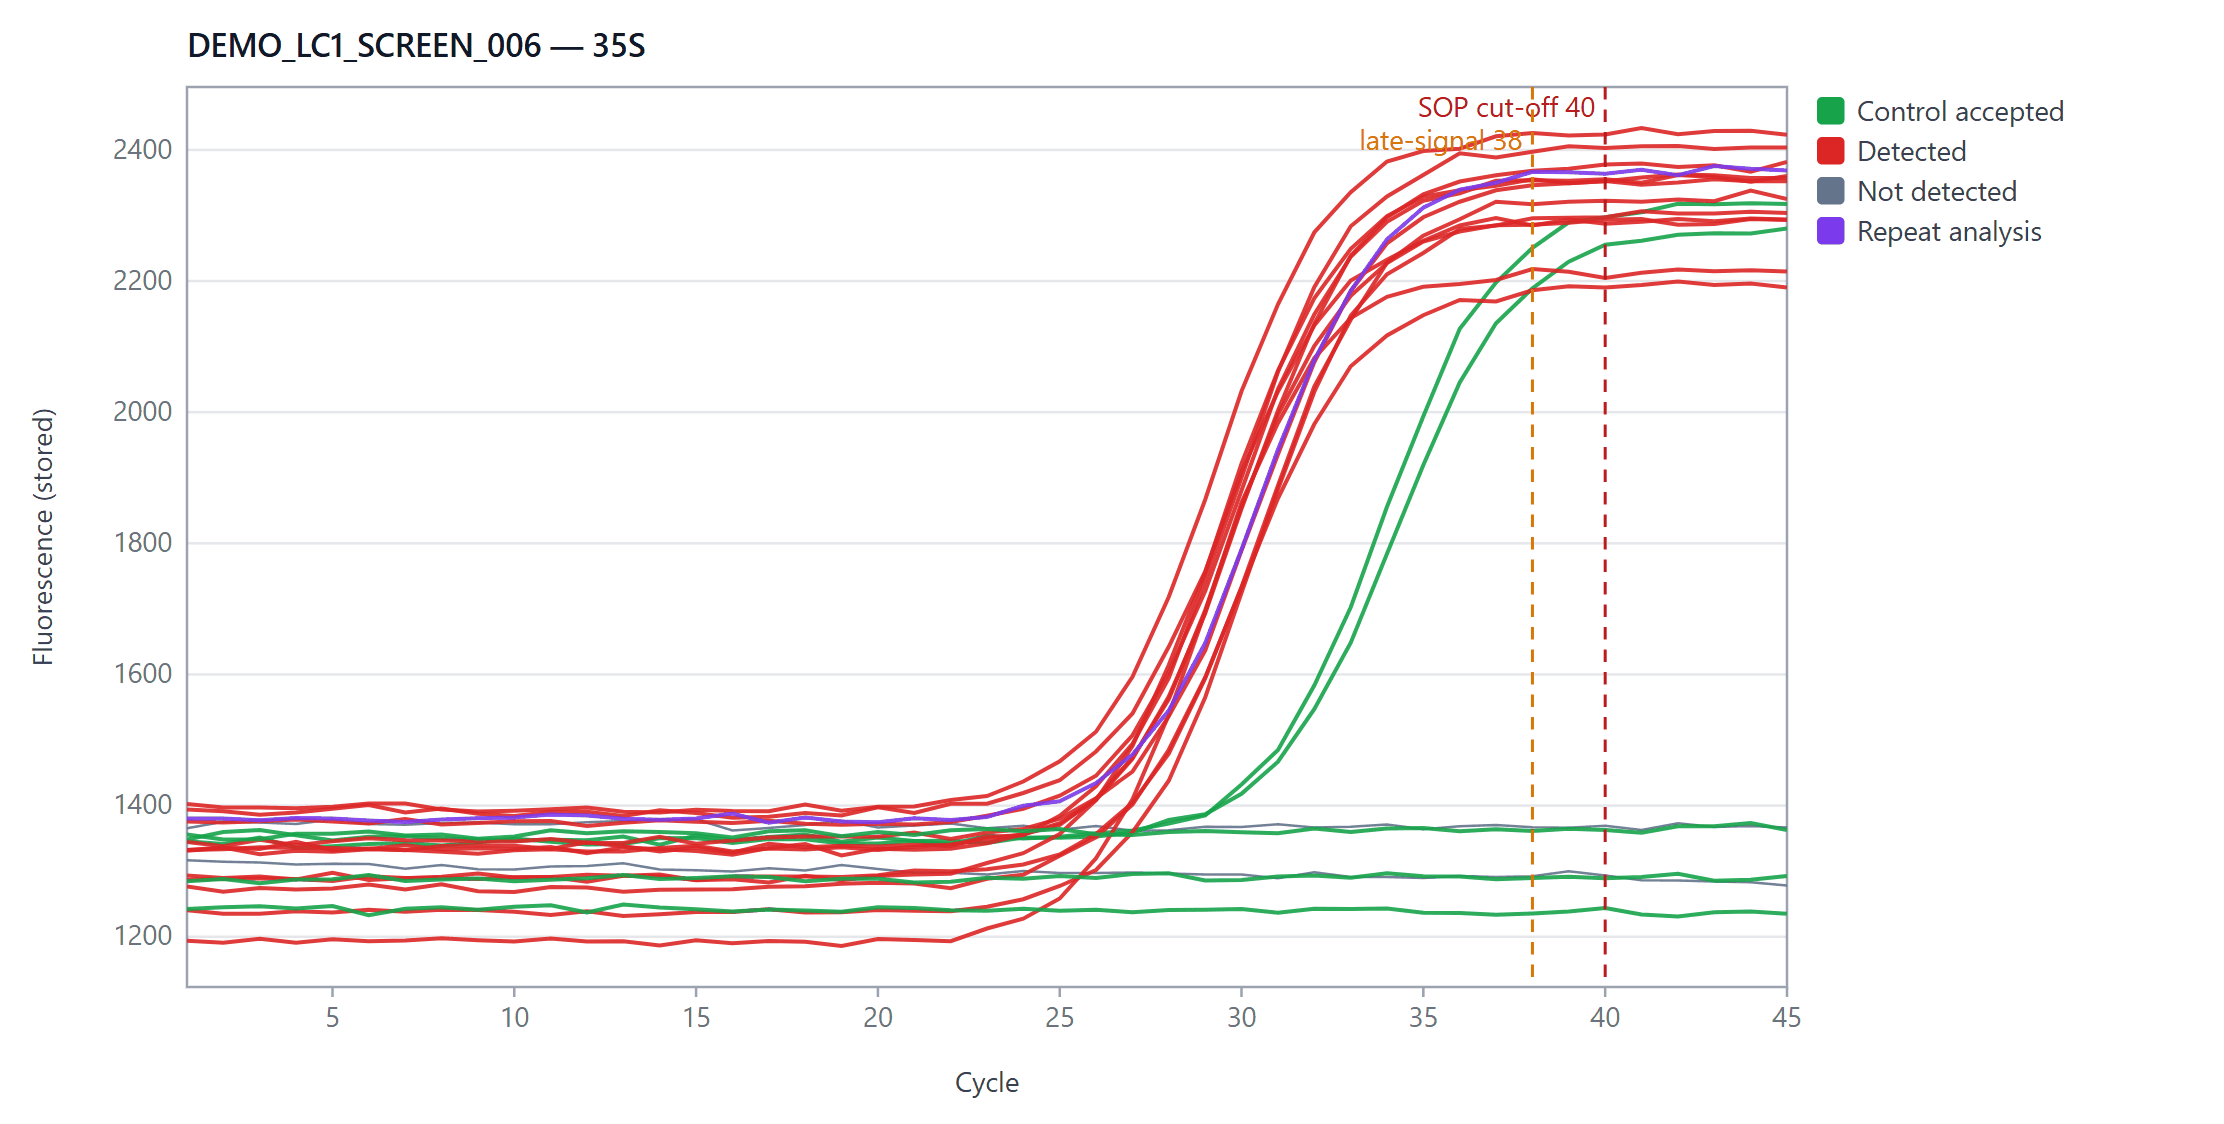
\includegraphics[width=\linewidth]{fig/g_LC_curves.png}\caption{.ixo instrument, 35S, accepted run}\label{fig:g_LC_curves}\end{subfigure}\hfill
\begin{subfigure}{0.49\linewidth}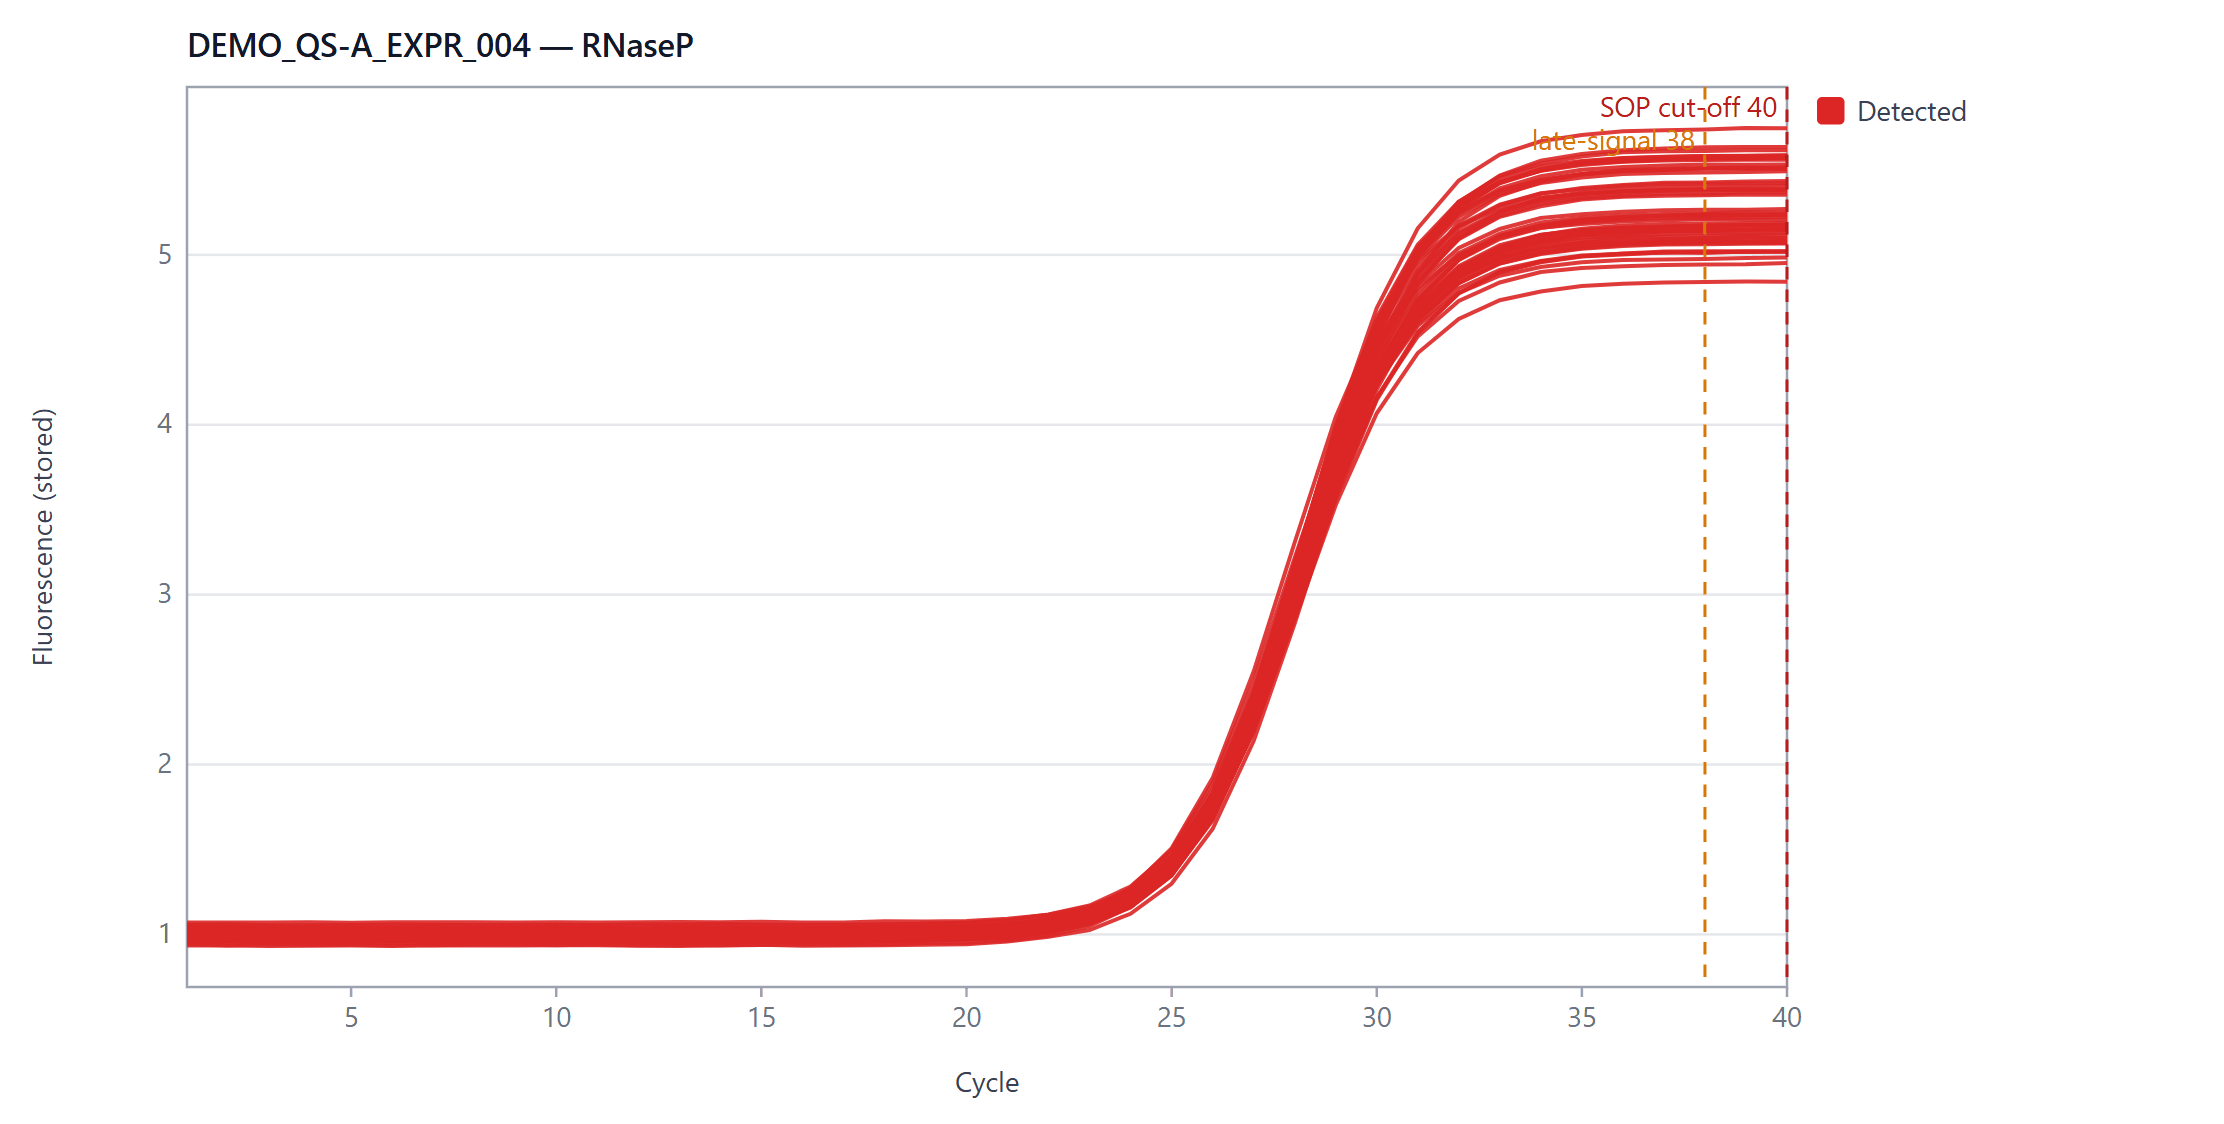
\includegraphics[width=\linewidth]{fig/g_QS_curves.png}\caption{.eds instrument, RAS}\label{fig:g_QS_curves}\end{subfigure}
\caption{\synthtag \texttt{curves} — amplification curves coloured by SOP outcome, with the SOP Cq cut-off and late-signal limit.}\label{fig:curves}
\end{figure}
\begin{figure}[htbp]\centering
\begin{subfigure}{0.49\linewidth}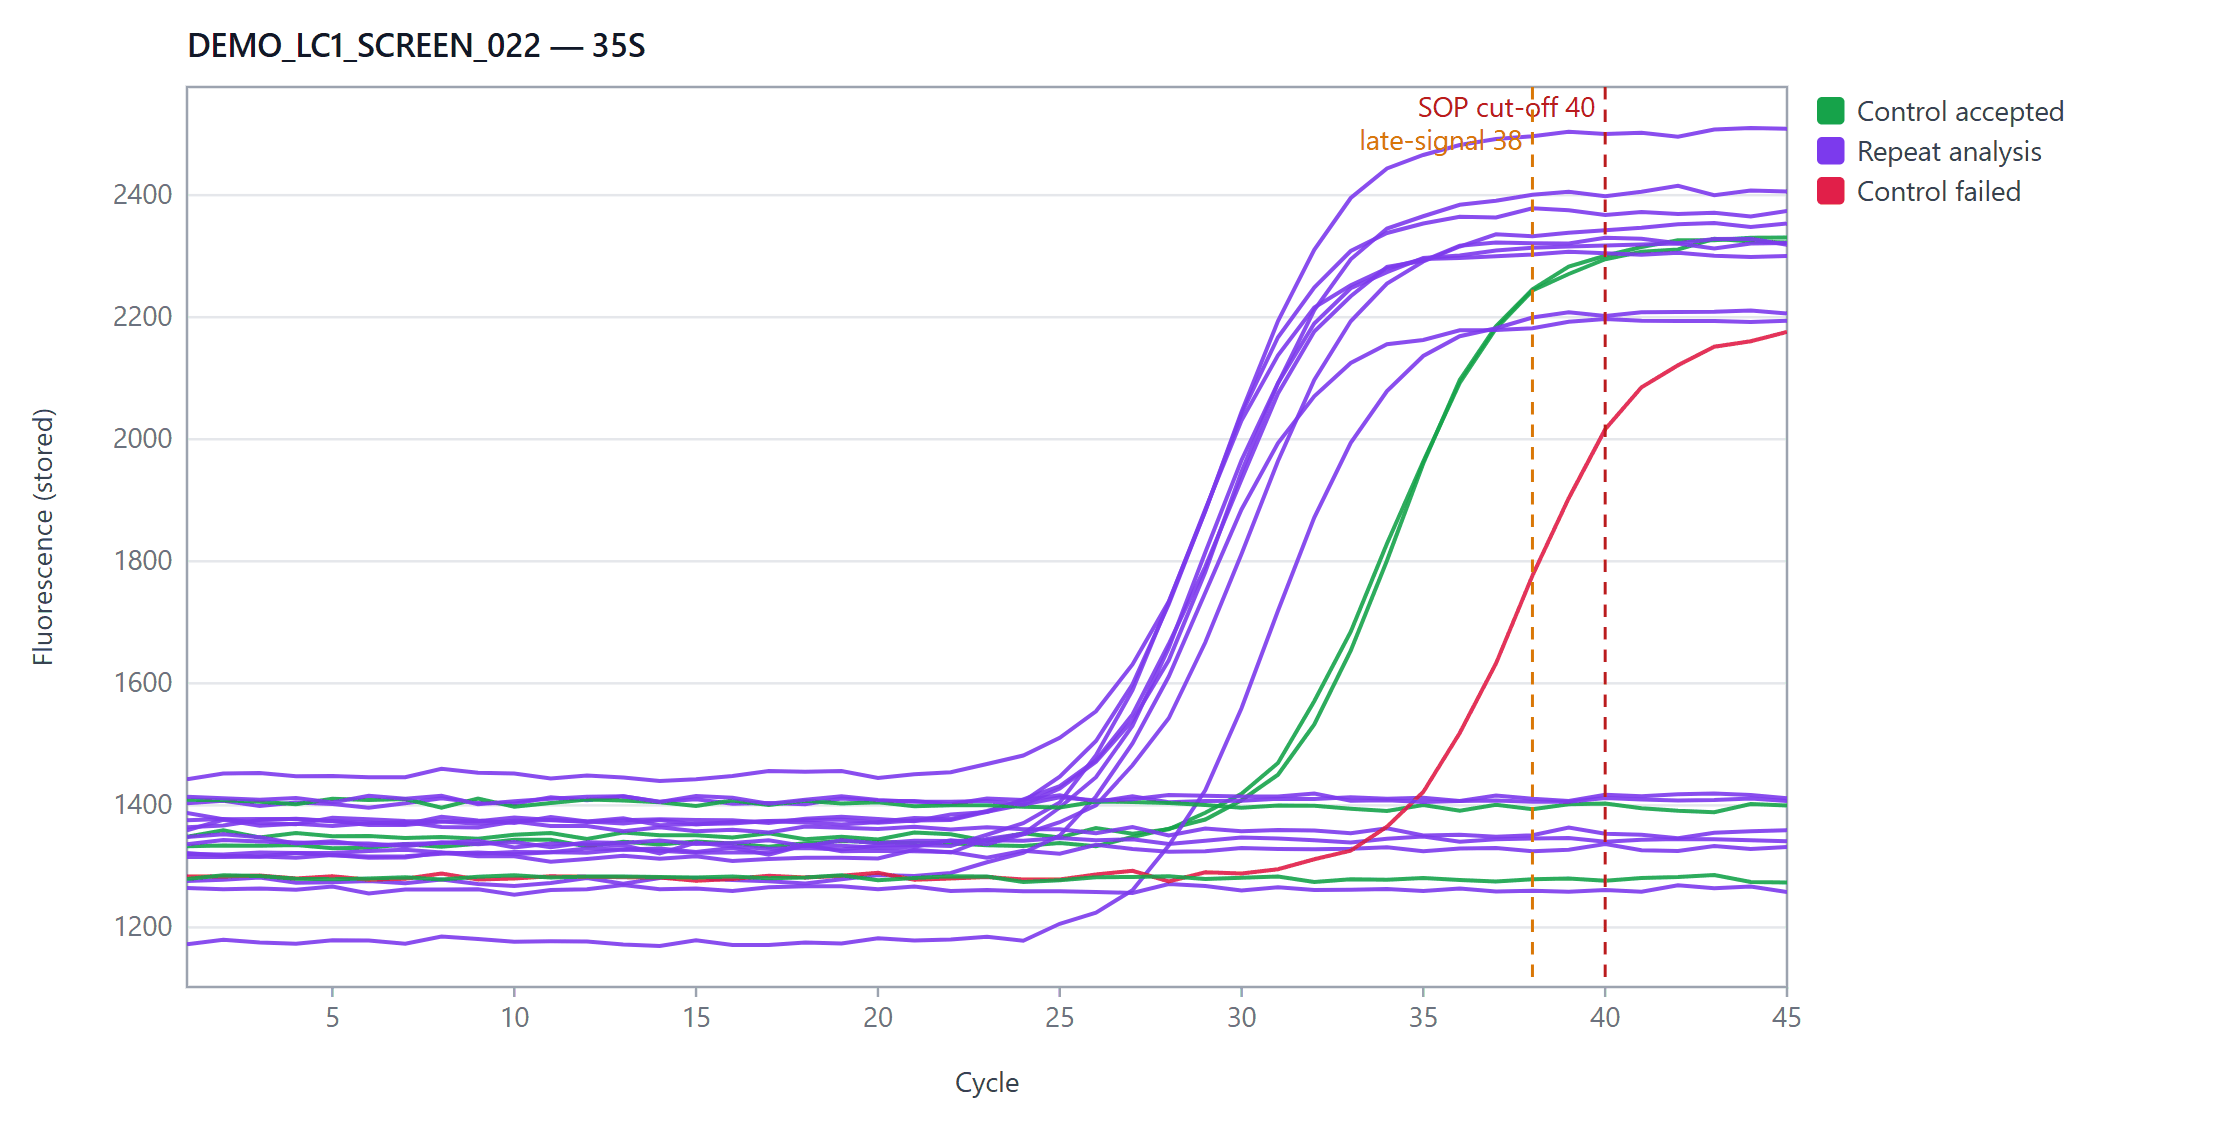
\includegraphics[width=\linewidth]{fig/g_LCX_curves.png}\caption{run 022: blank amplifies, run rejected}\label{fig:g_LCX_curves}\end{subfigure}\hfill
\begin{subfigure}{0.49\linewidth}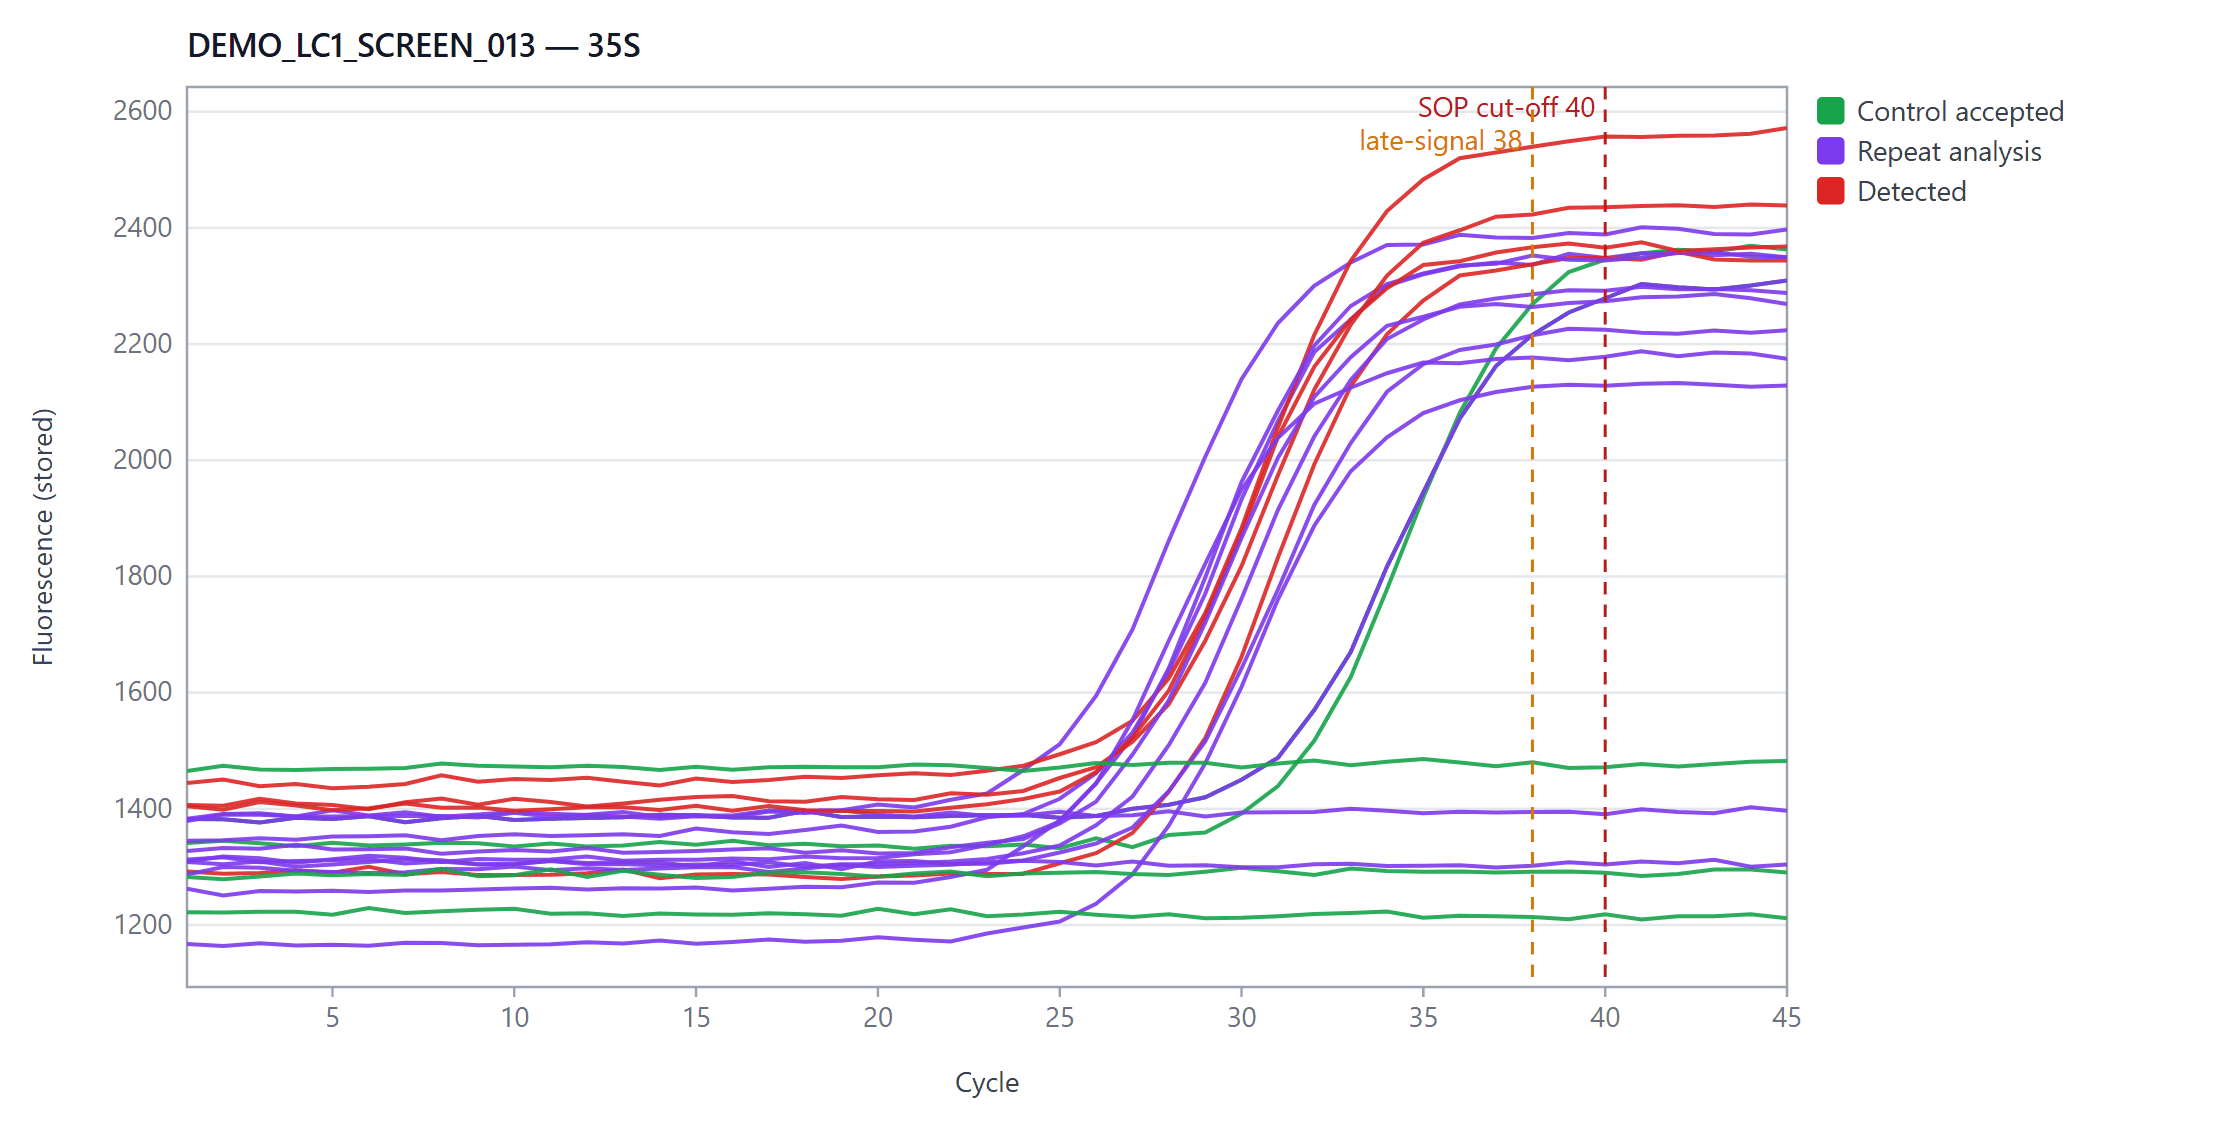
\includegraphics[width=\linewidth]{fig/g_LCC_curves.png}\caption{run 013: A03 is a copy of A01}\label{fig:g_LCC_curves}\end{subfigure}
\caption{\synthtag The planted events as the curves show them. In (a) the contaminated extraction blank (red, Cq 35.6) turns every result of the run into \emph{Invalid run}; in (b) two curves are identical point for point.}\label{fig:planted_curves}
\end{figure}
\fig[0.85]{g_QC_curves.png}{\texttt{curves} for a 10-point dilution series (\texttt{DEMO\_QS-C\_STDCURVE\_002}).}{g_QC_curves}
\fig[0.85]{g_LC_unanalysed.png}{\texttt{unanalysed} — curves of wells that are in no analysis. A signal here is a result nobody looked at.}{g_LC_unanalysed}
\begin{figure}[htbp]\centering
\begin{subfigure}{0.49\linewidth}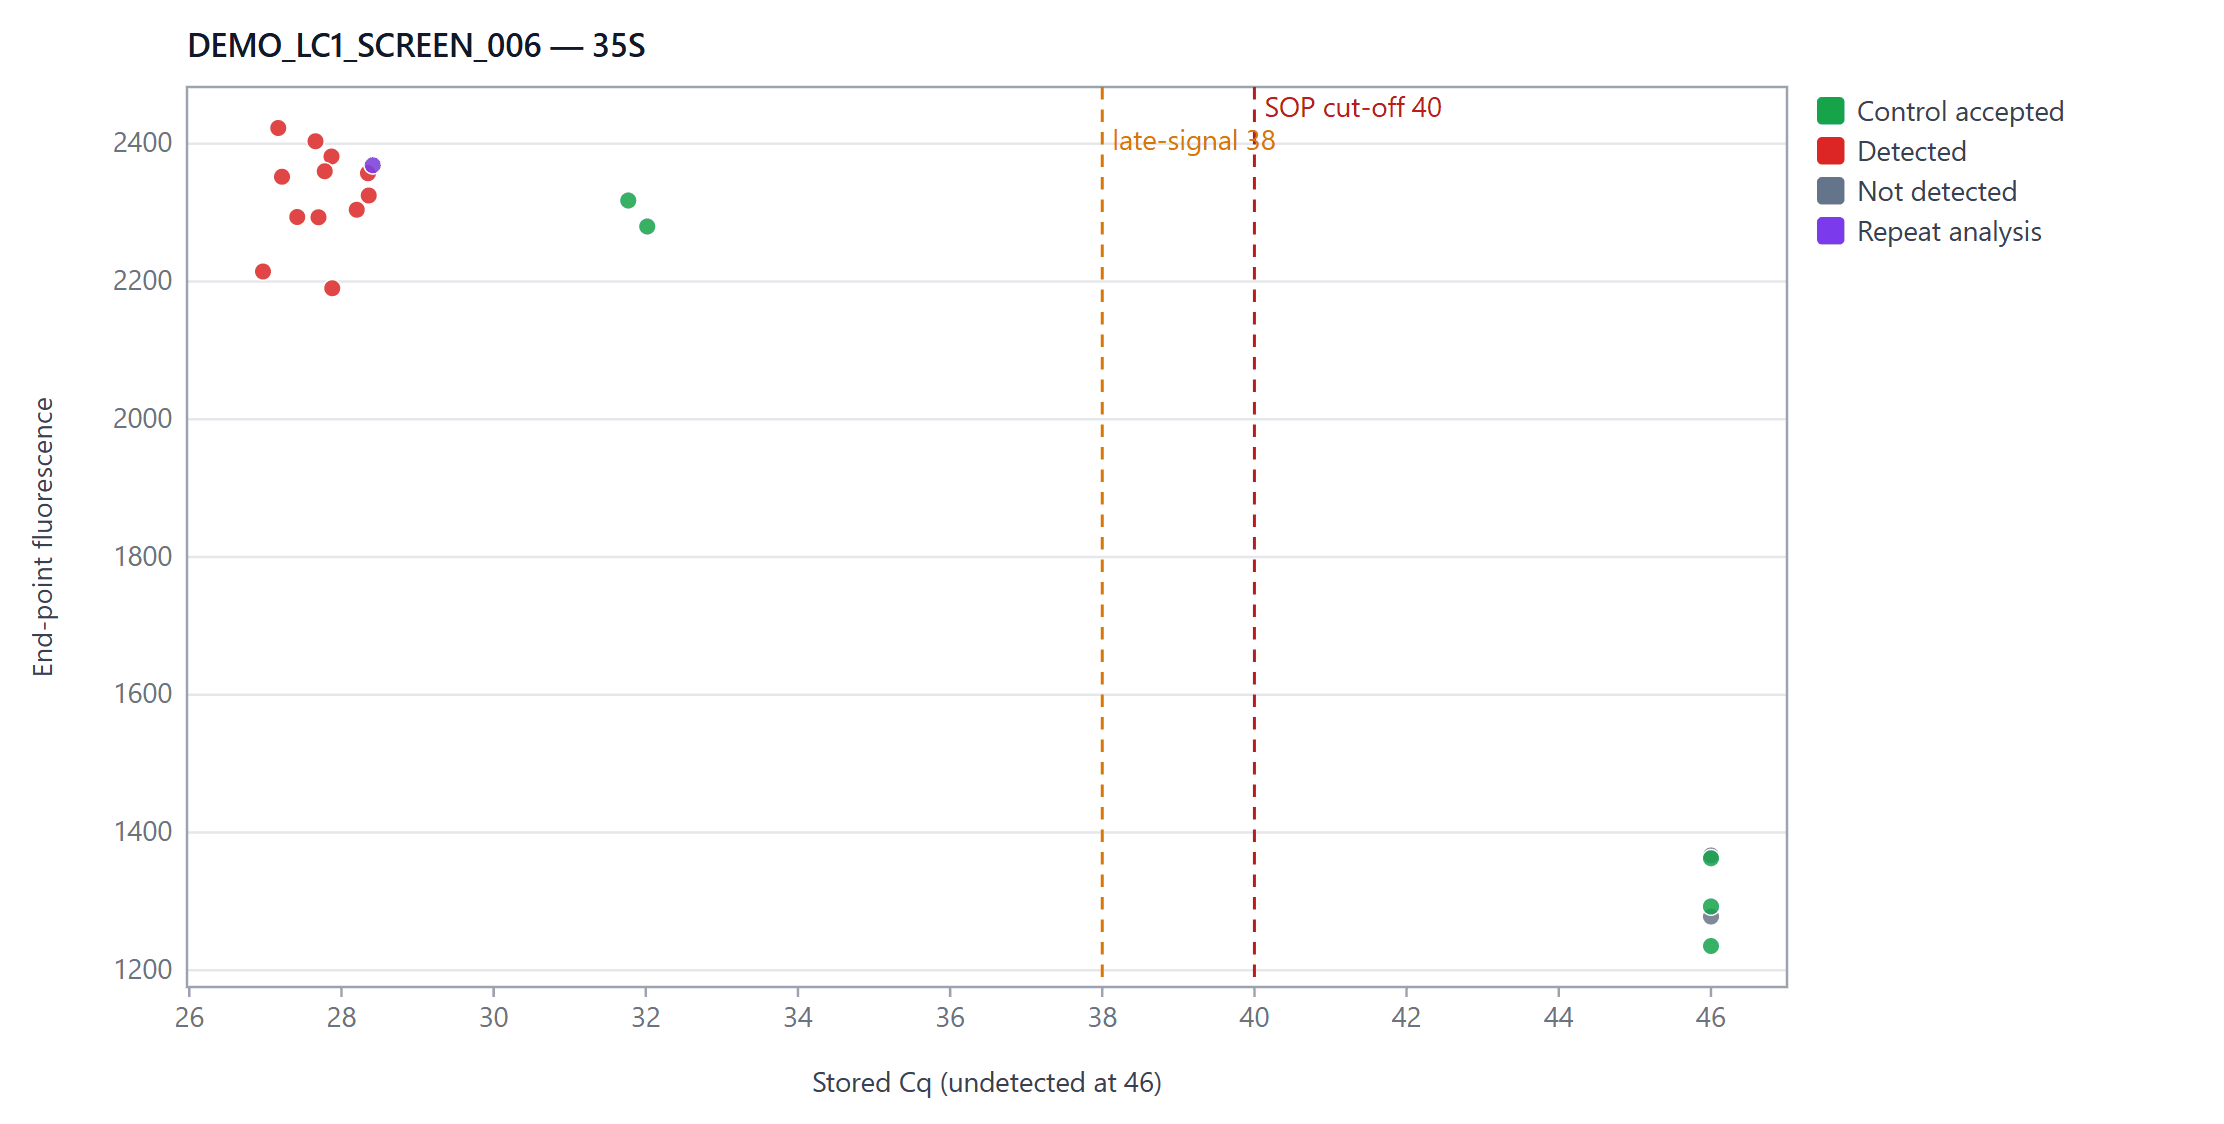
\includegraphics[width=\linewidth]{fig/g_LC_endpoint.png}\caption{\texttt{endpoint}: fluorescence against Cq}\end{subfigure}\hfill
\begin{subfigure}{0.49\linewidth}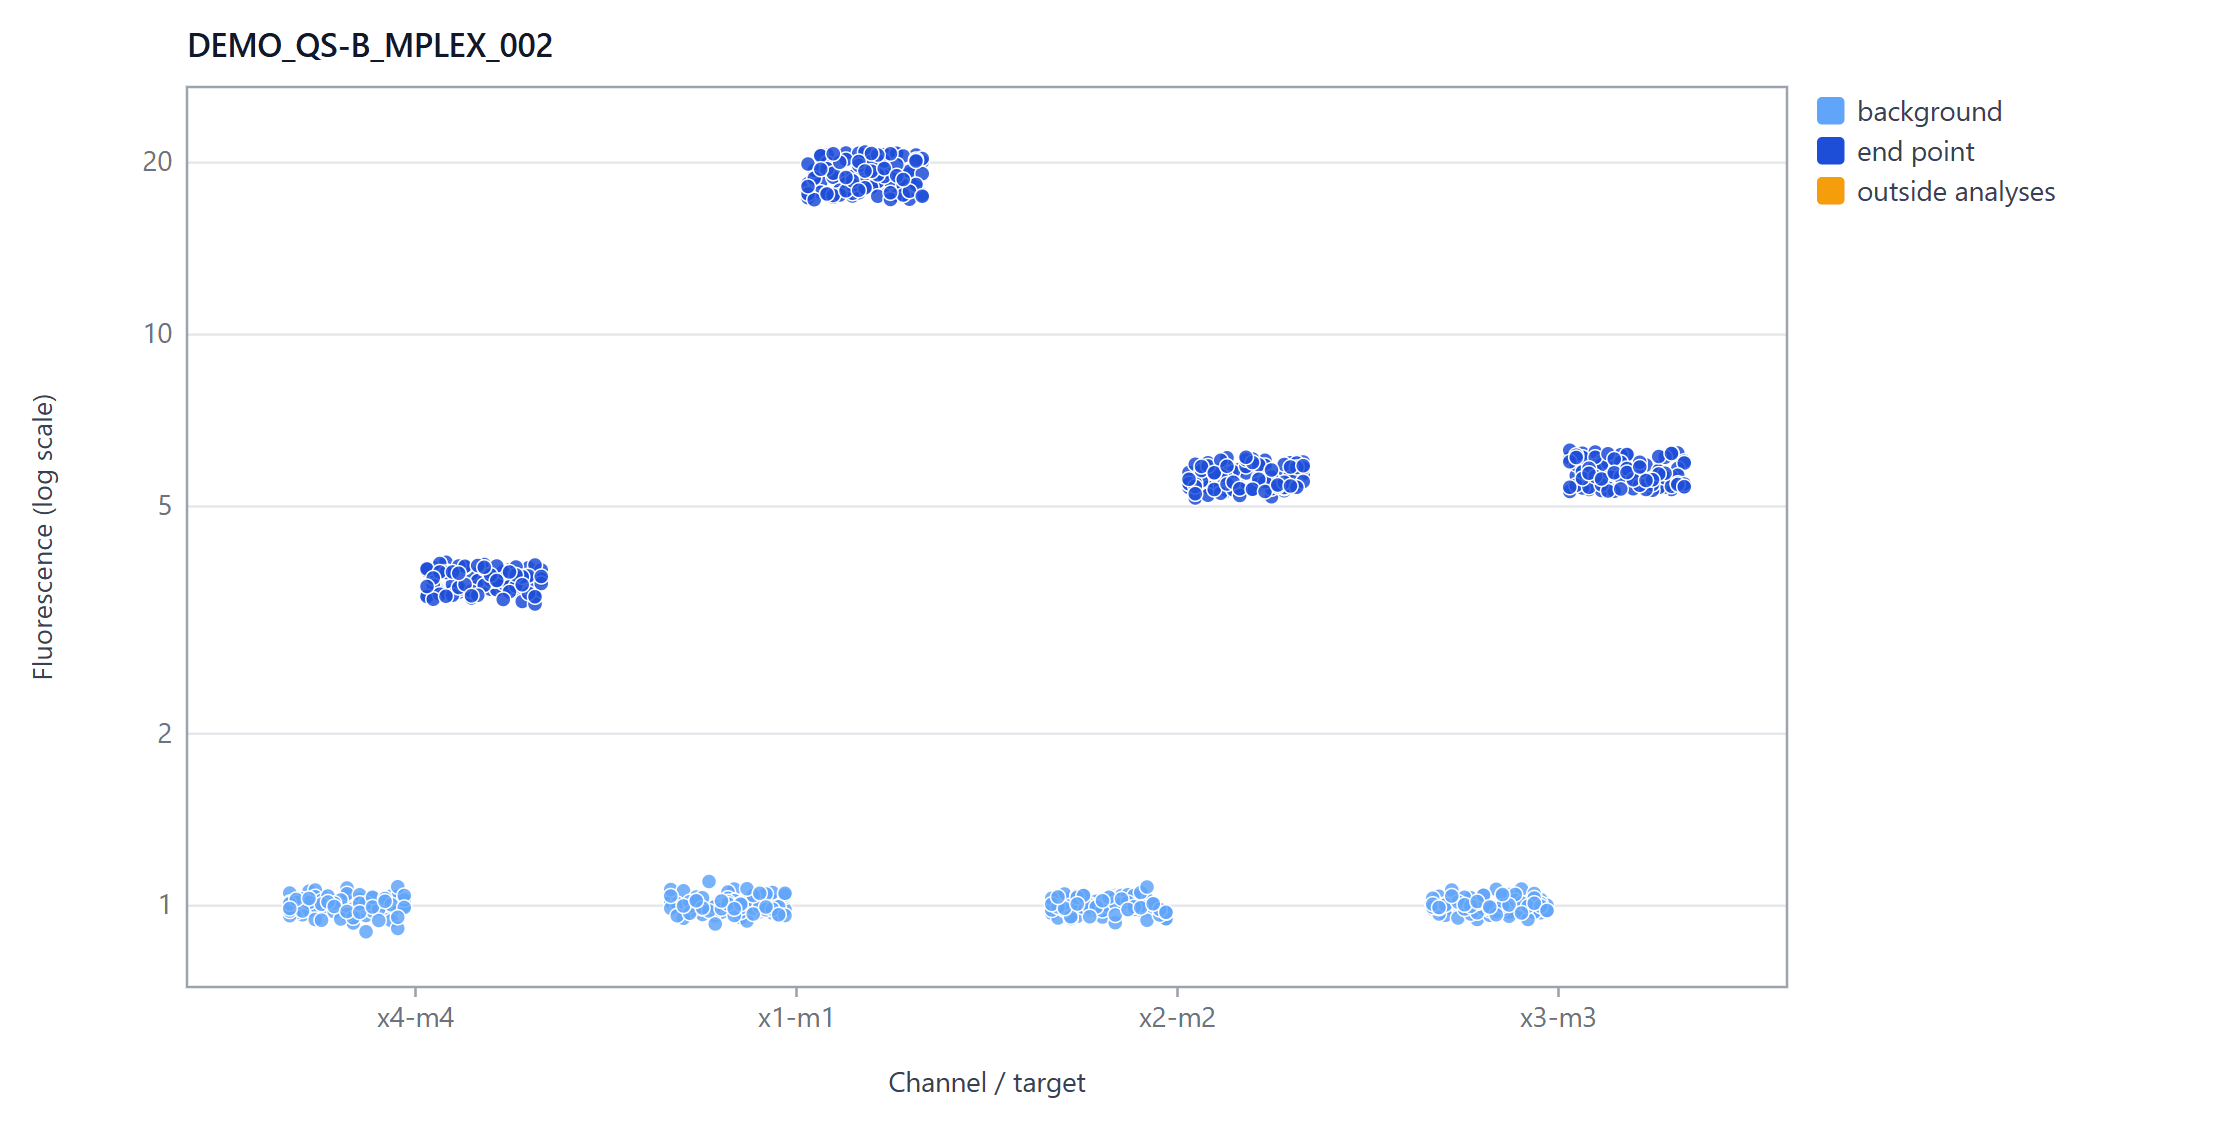
\includegraphics[width=\linewidth]{fig/g_QB_levels.png}\caption{\texttt{levels}: background and plateau per channel}\end{subfigure}
\caption{\synthtag Signal level graphs.}\label{fig:levels}
\end{figure}

\subsection*{Plate and results}
\begin{figure}[htbp]\centering
\begin{subfigure}{0.49\linewidth}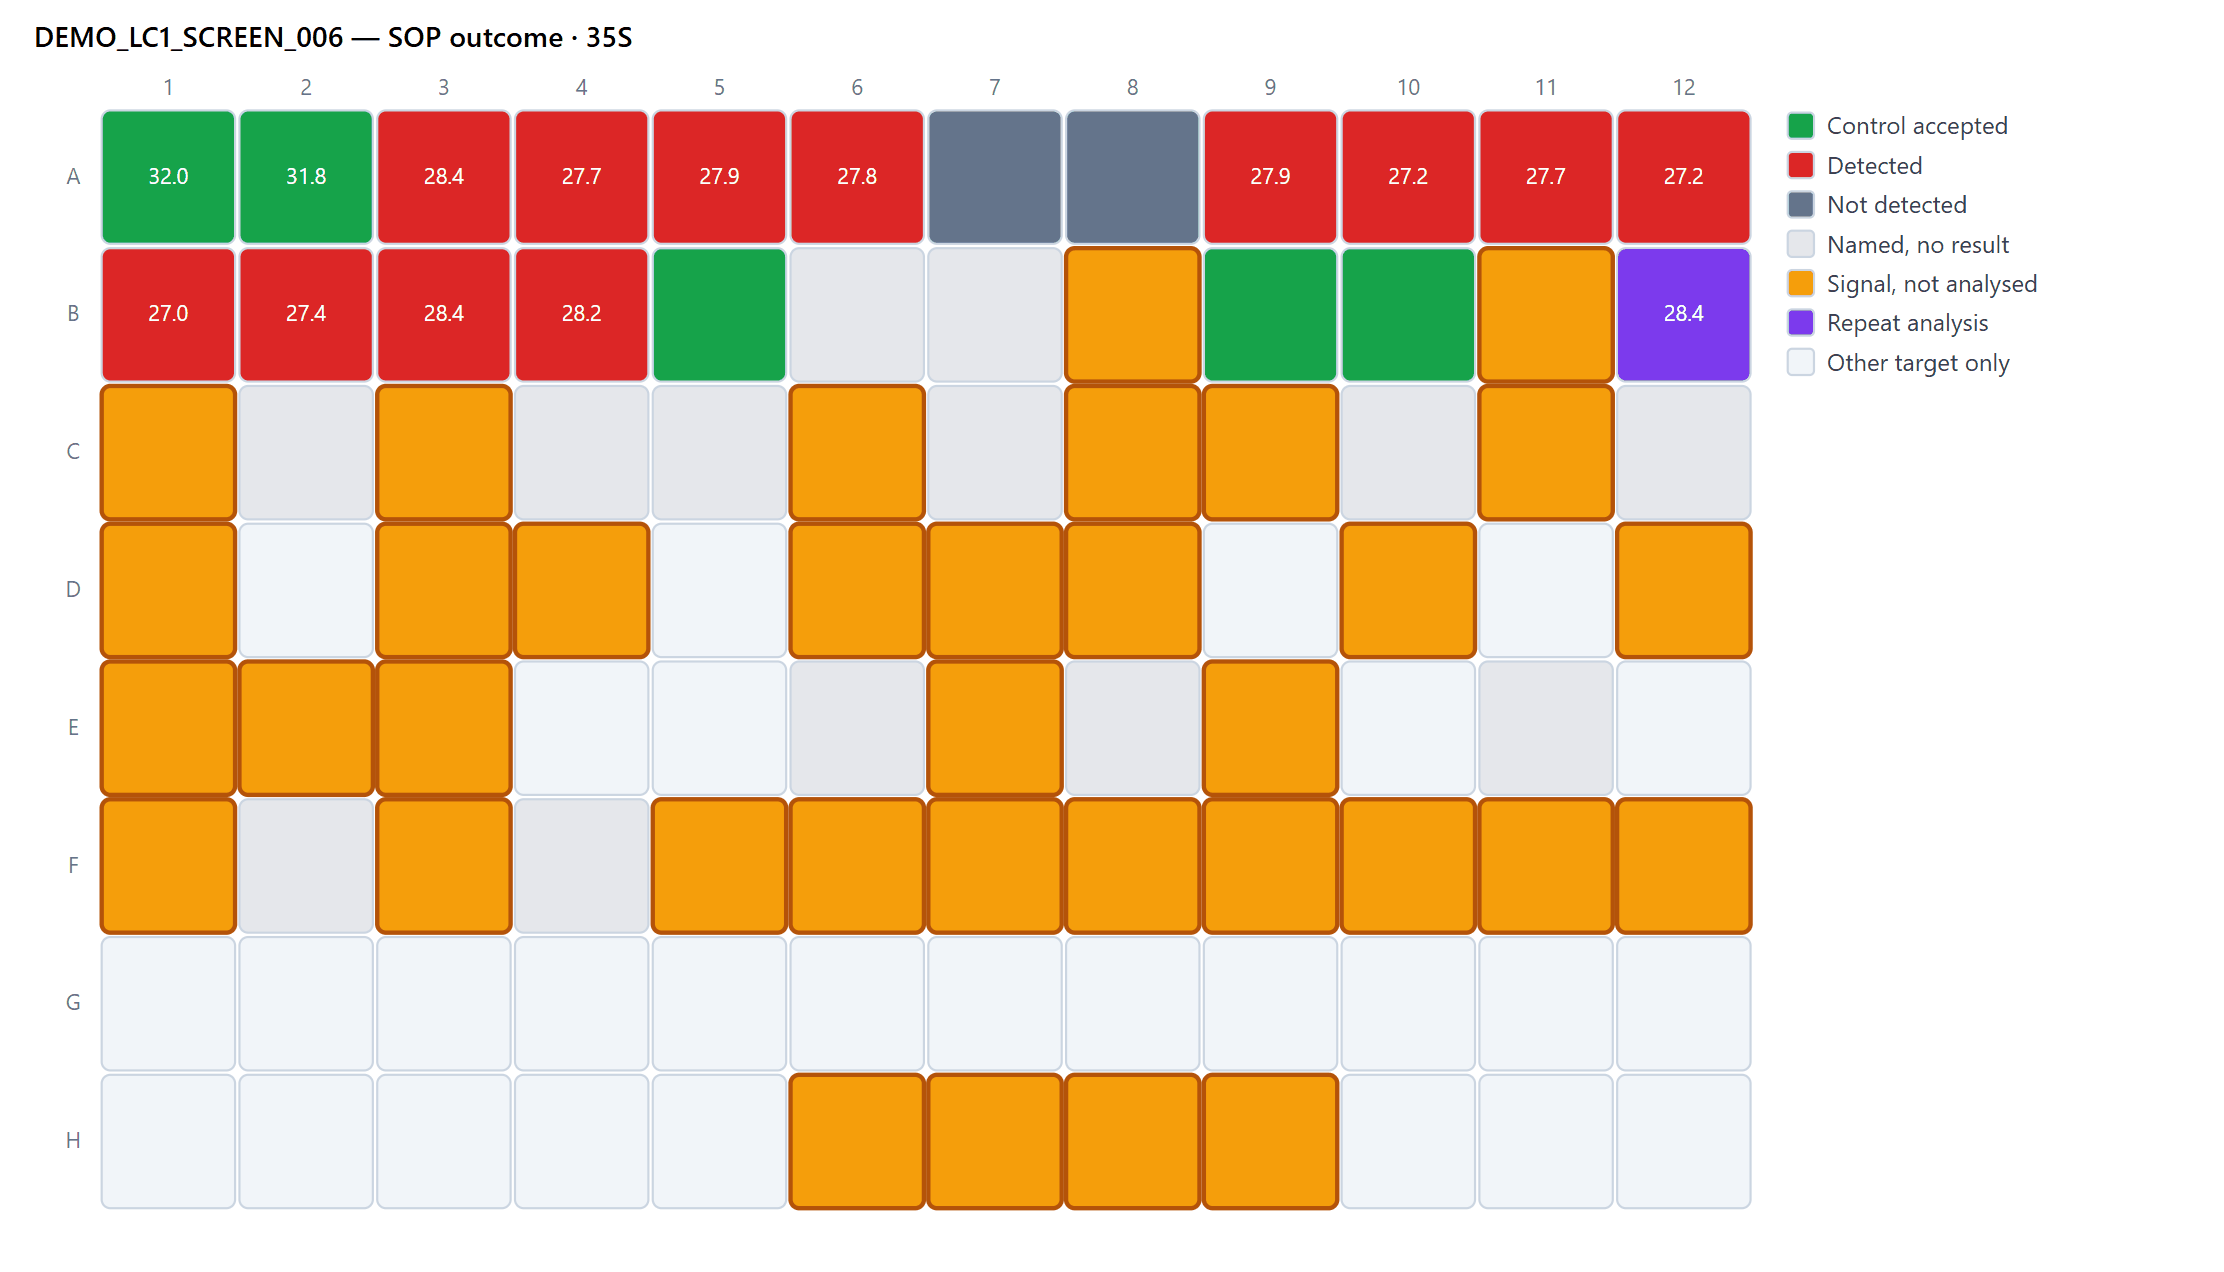
\includegraphics[width=\linewidth]{fig/g_LC_plate.png}\caption{.ixo instrument, 35S}\end{subfigure}\hfill
\begin{subfigure}{0.49\linewidth}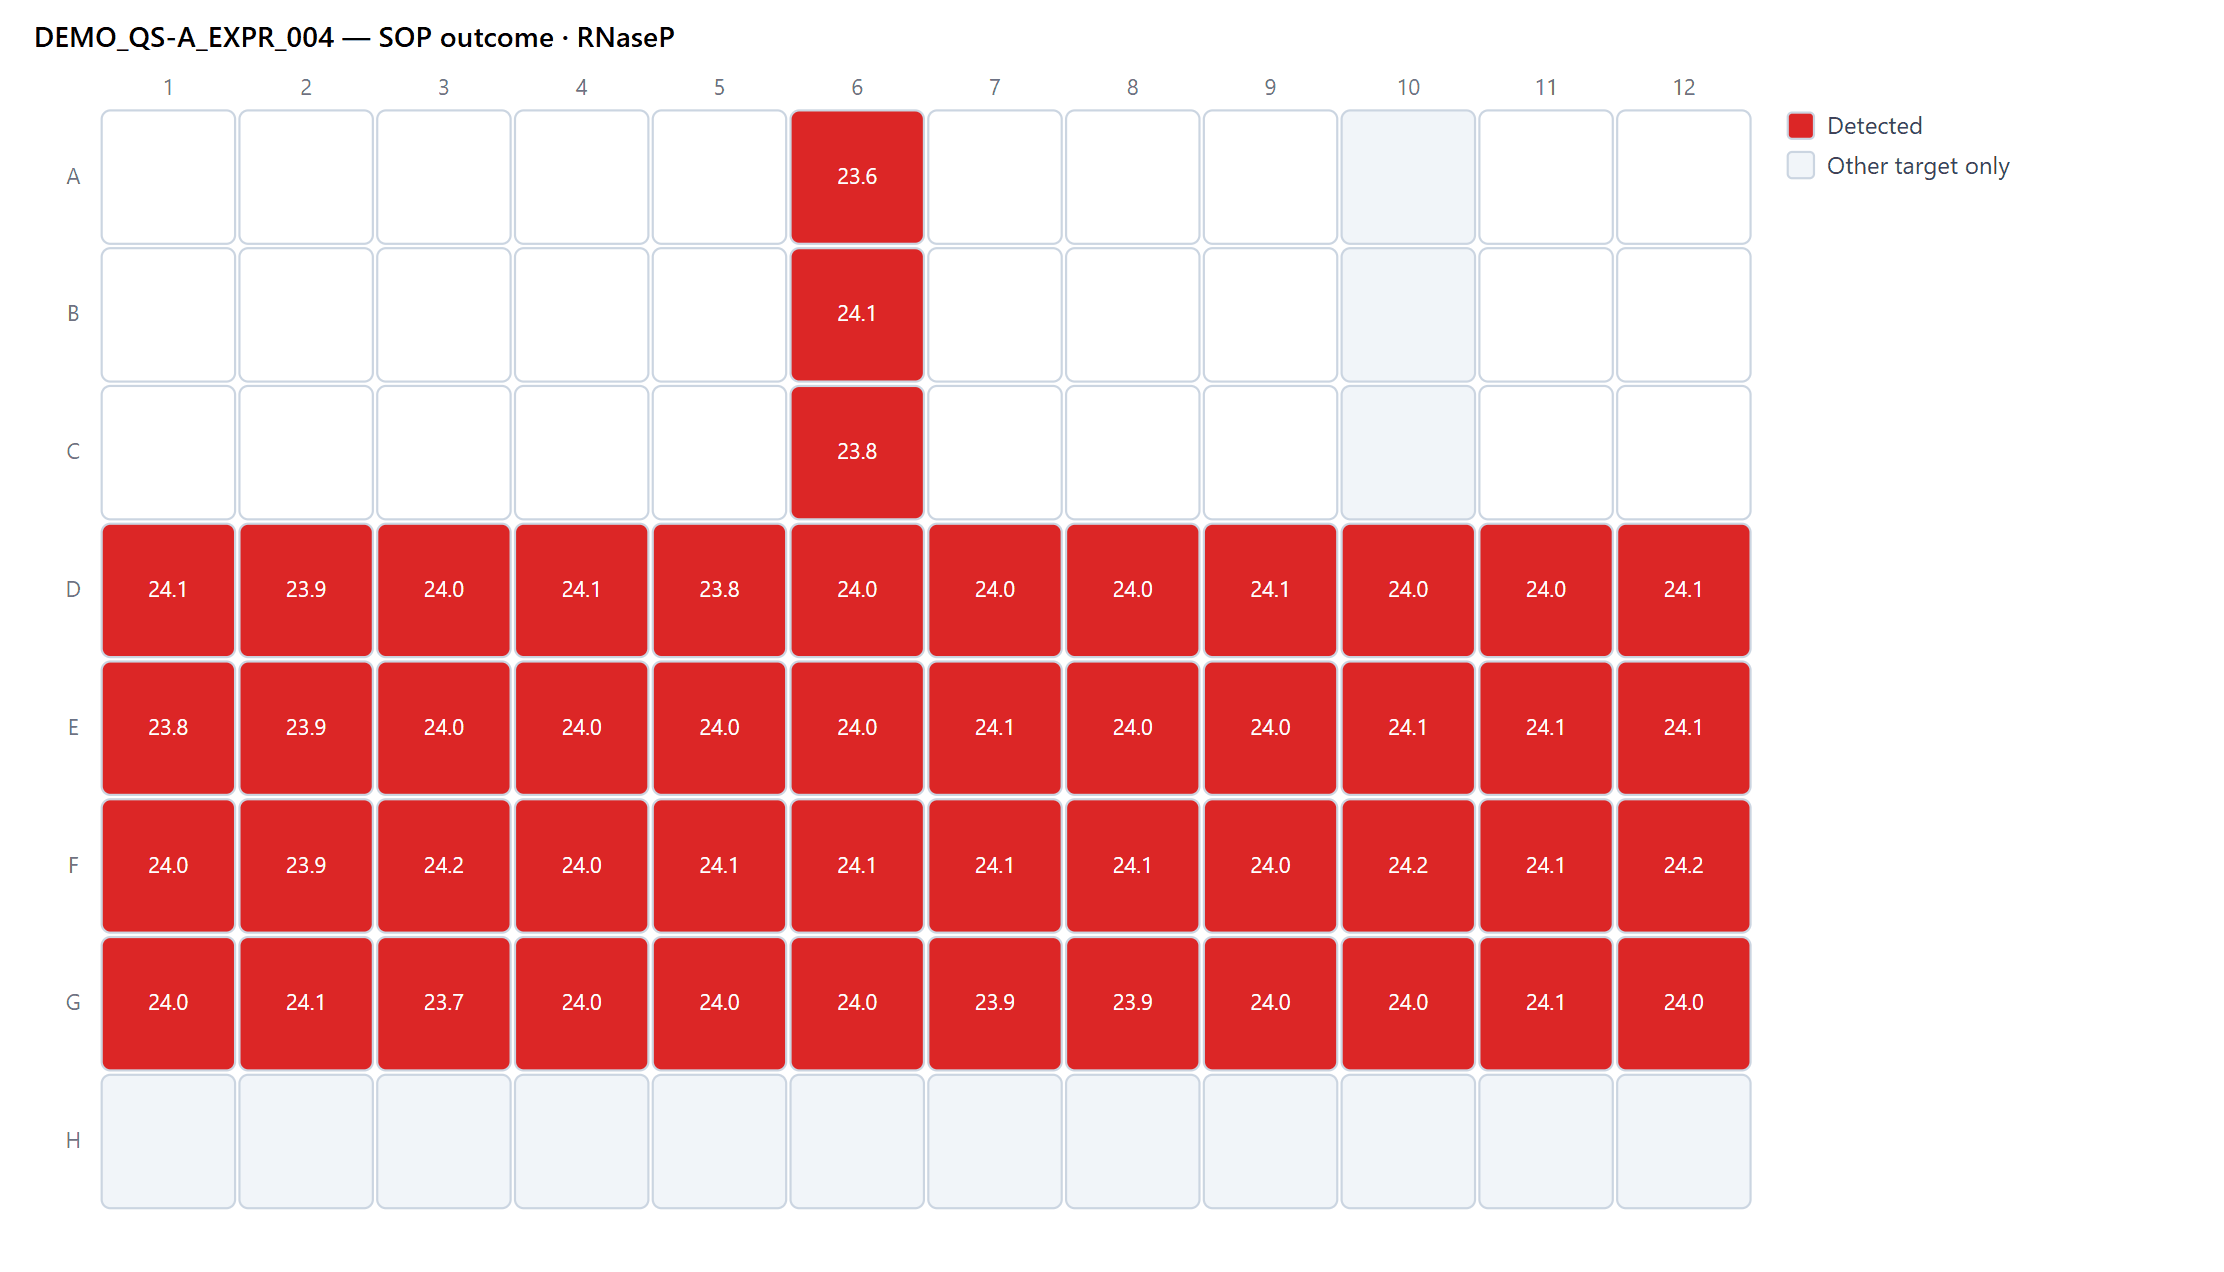
\includegraphics[width=\linewidth]{fig/g_QS_plate.png}\caption{.eds instrument, RAS}\end{subfigure}
\caption{\synthtag \texttt{plate} — heat map of the SOP outcome per well, with the stored Cq. Wells with a signal that is not analysed are outlined.}\label{fig:plate}
\end{figure}
\begin{figure}[htbp]\centering
\begin{subfigure}{0.49\linewidth}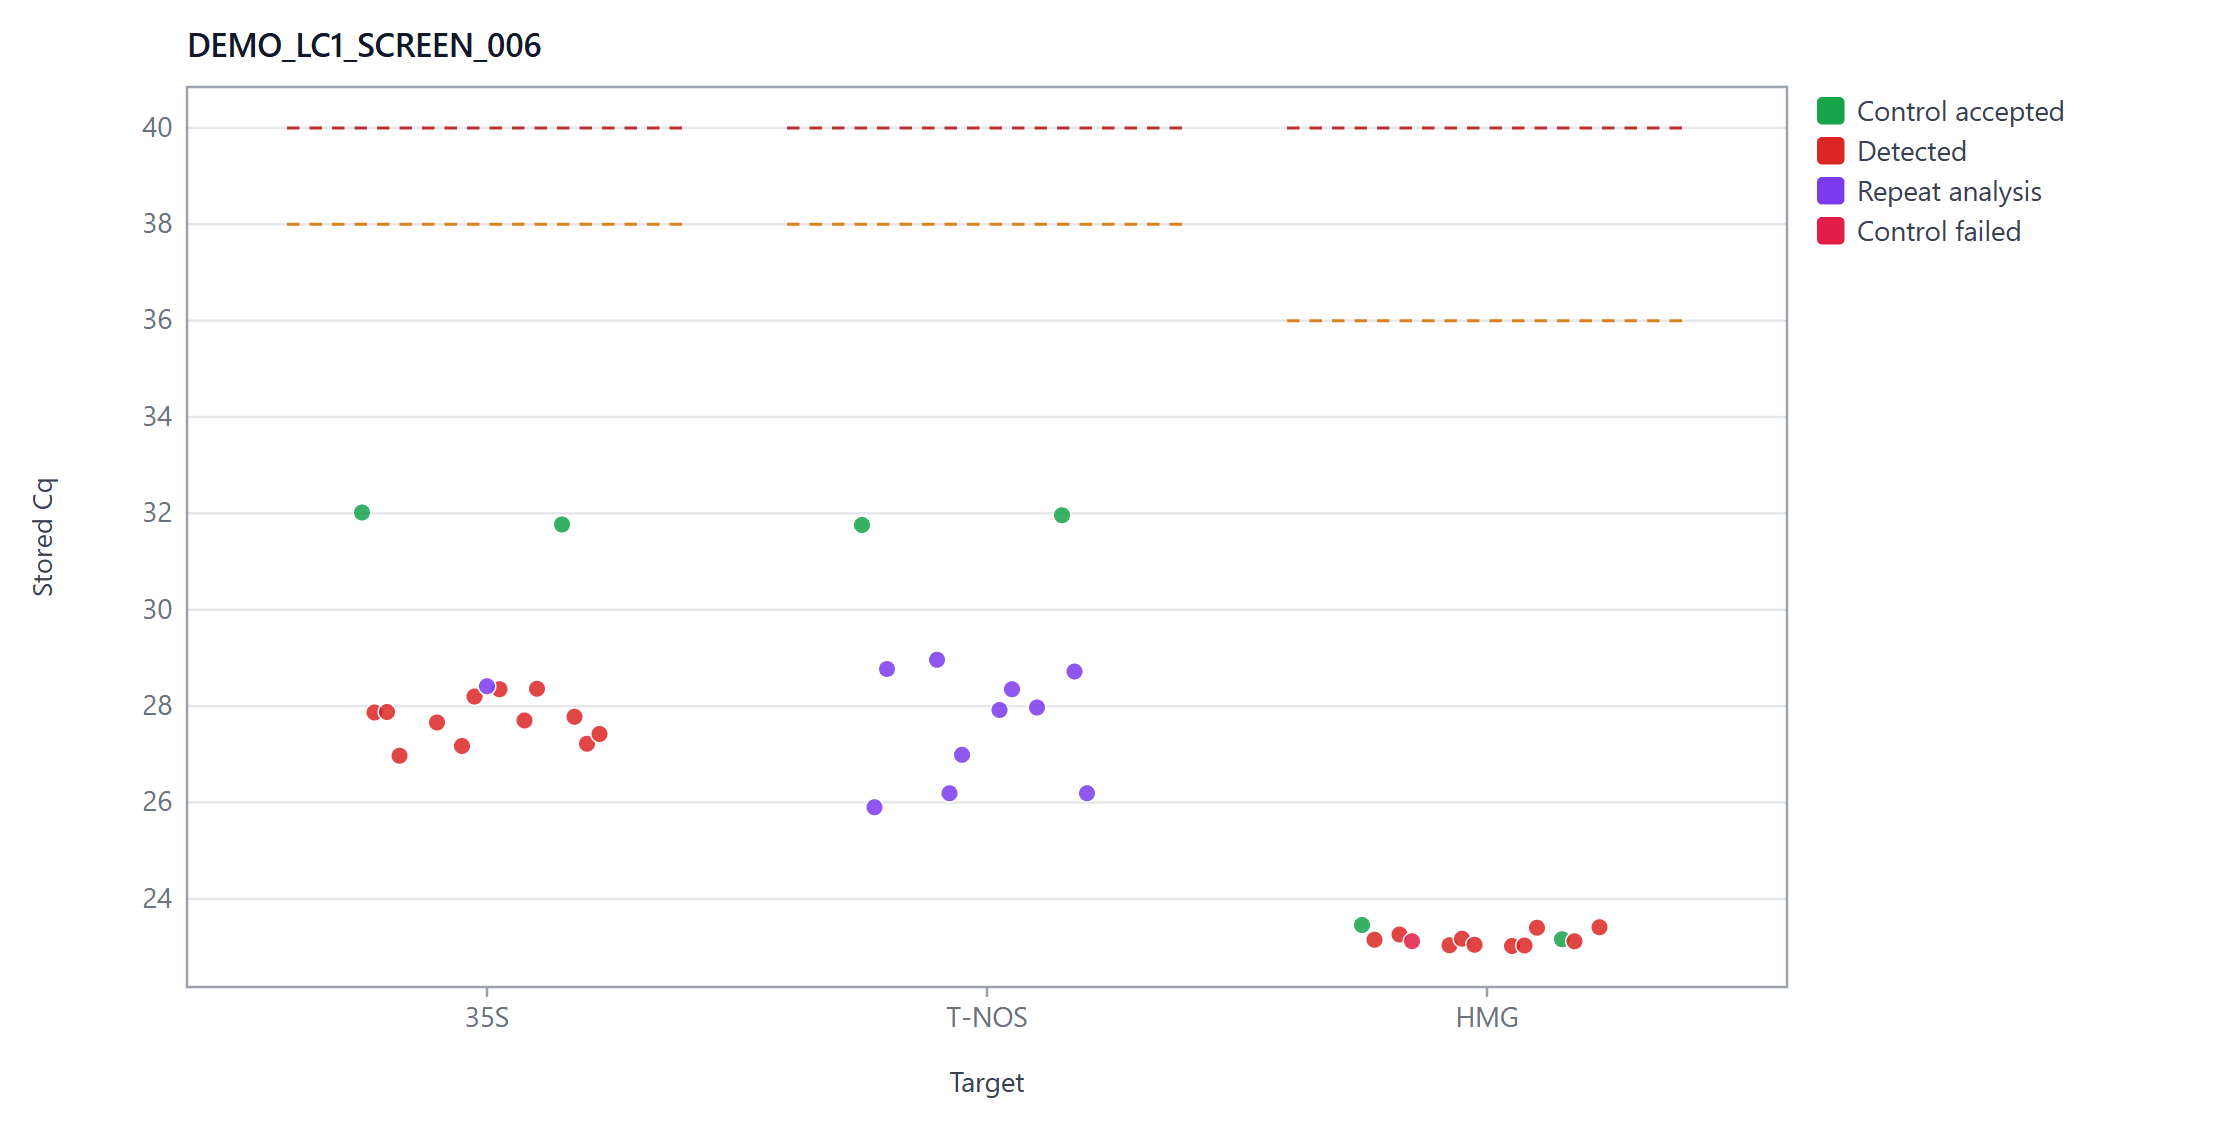
\includegraphics[width=\linewidth]{fig/g_LC_cqstrip.png}\caption{\texttt{cqstrip}}\end{subfigure}\hfill
\begin{subfigure}{0.49\linewidth}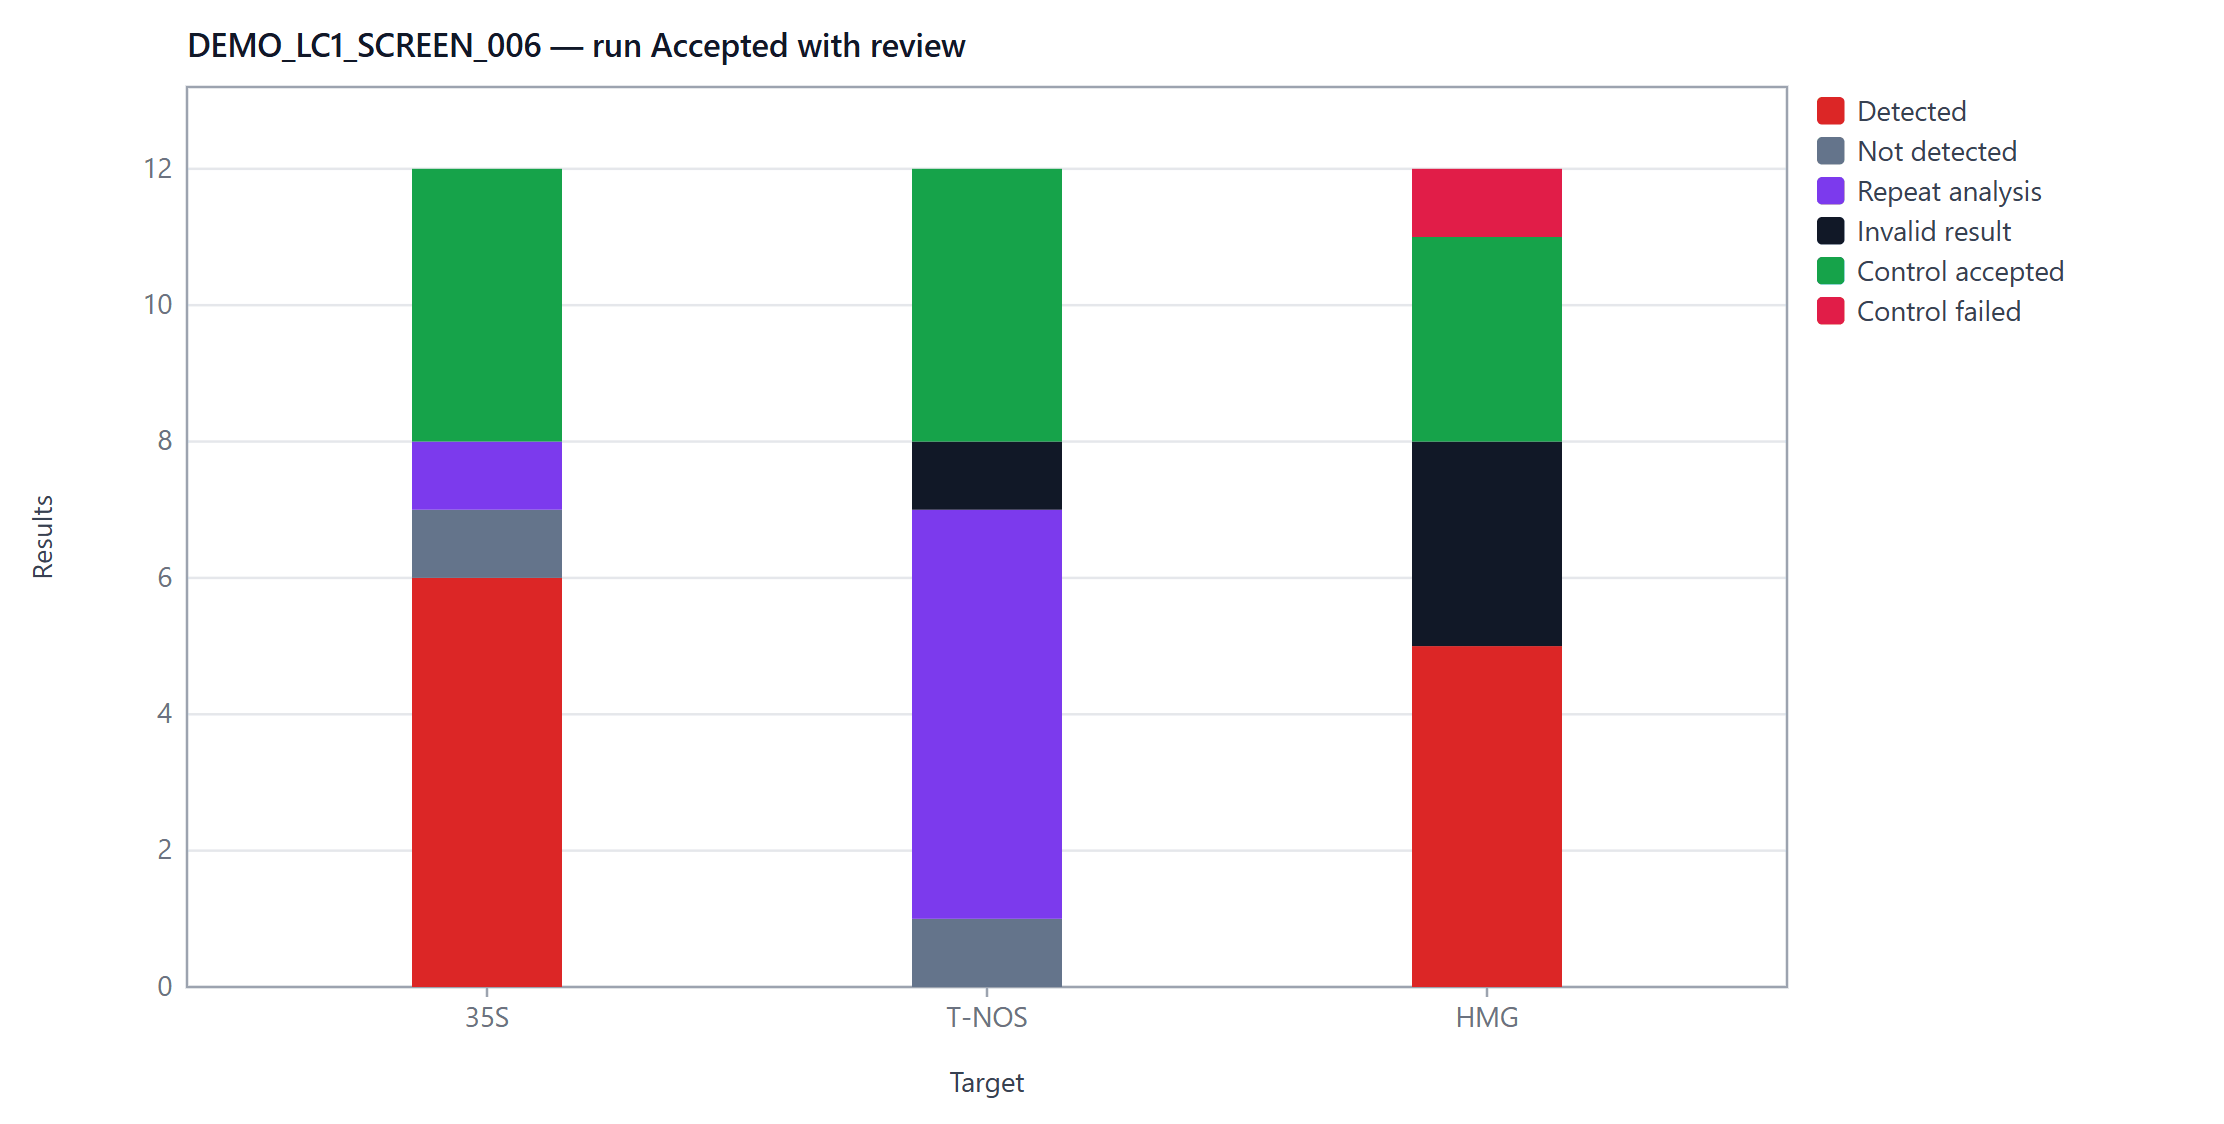
\includegraphics[width=\linewidth]{fig/g_LC_outcomes.png}\caption{\texttt{outcomes}}\end{subfigure}
\caption{\synthtag Cq by target with the SOP cut-offs, and SOP outcomes per target (\texttt{DEMO\_LC1\_SCREEN\_006}).}\label{fig:cqstrip}
\end{figure}
\begin{figure}[htbp]\centering
\begin{subfigure}{0.49\linewidth}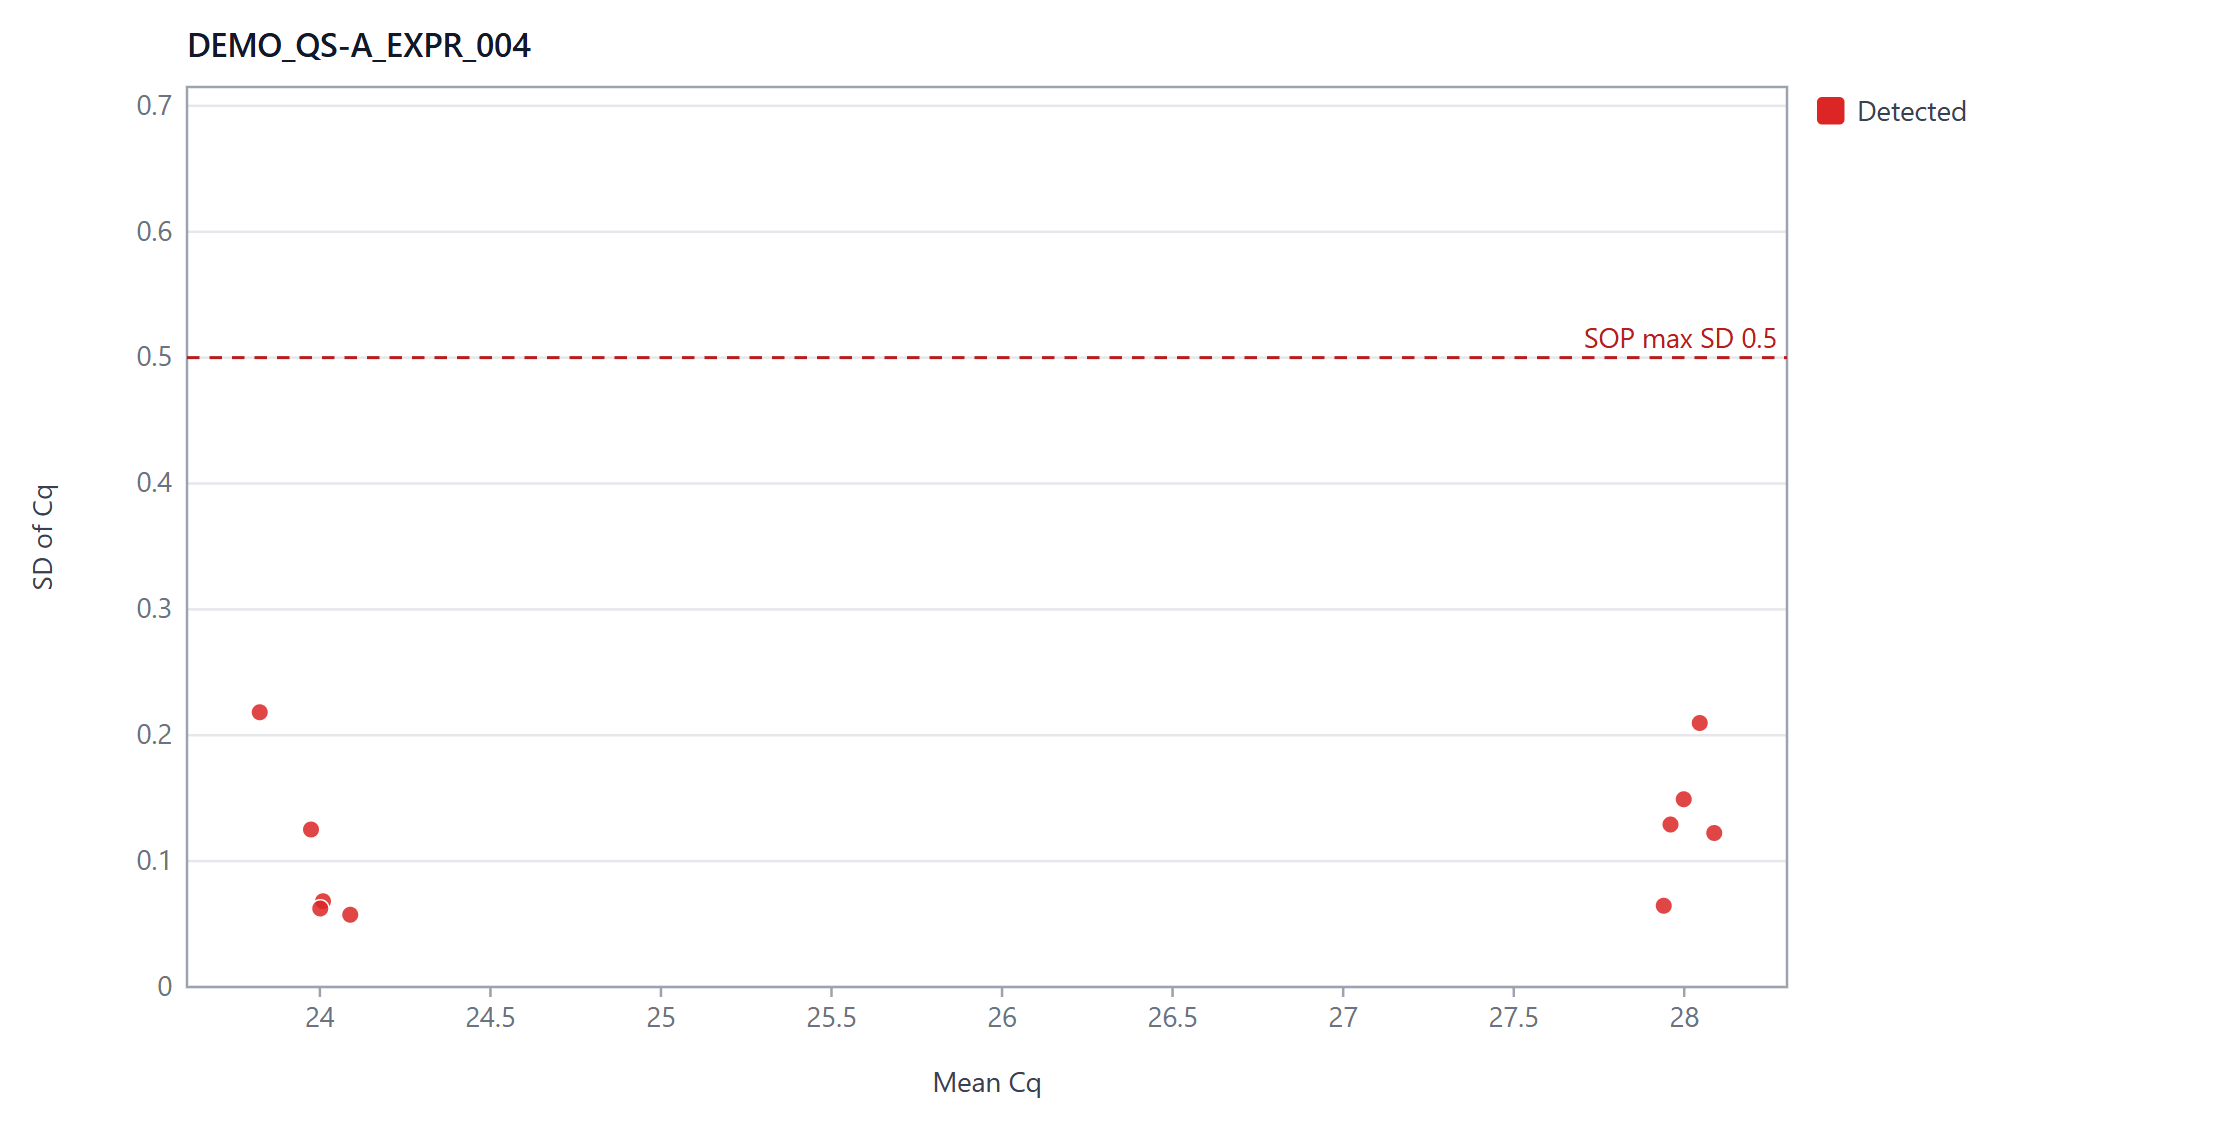
\includegraphics[width=\linewidth]{fig/g_QS_repsd.png}\caption{\texttt{repsd}: replicate SD against mean Cq}\end{subfigure}\hfill
\begin{subfigure}{0.49\linewidth}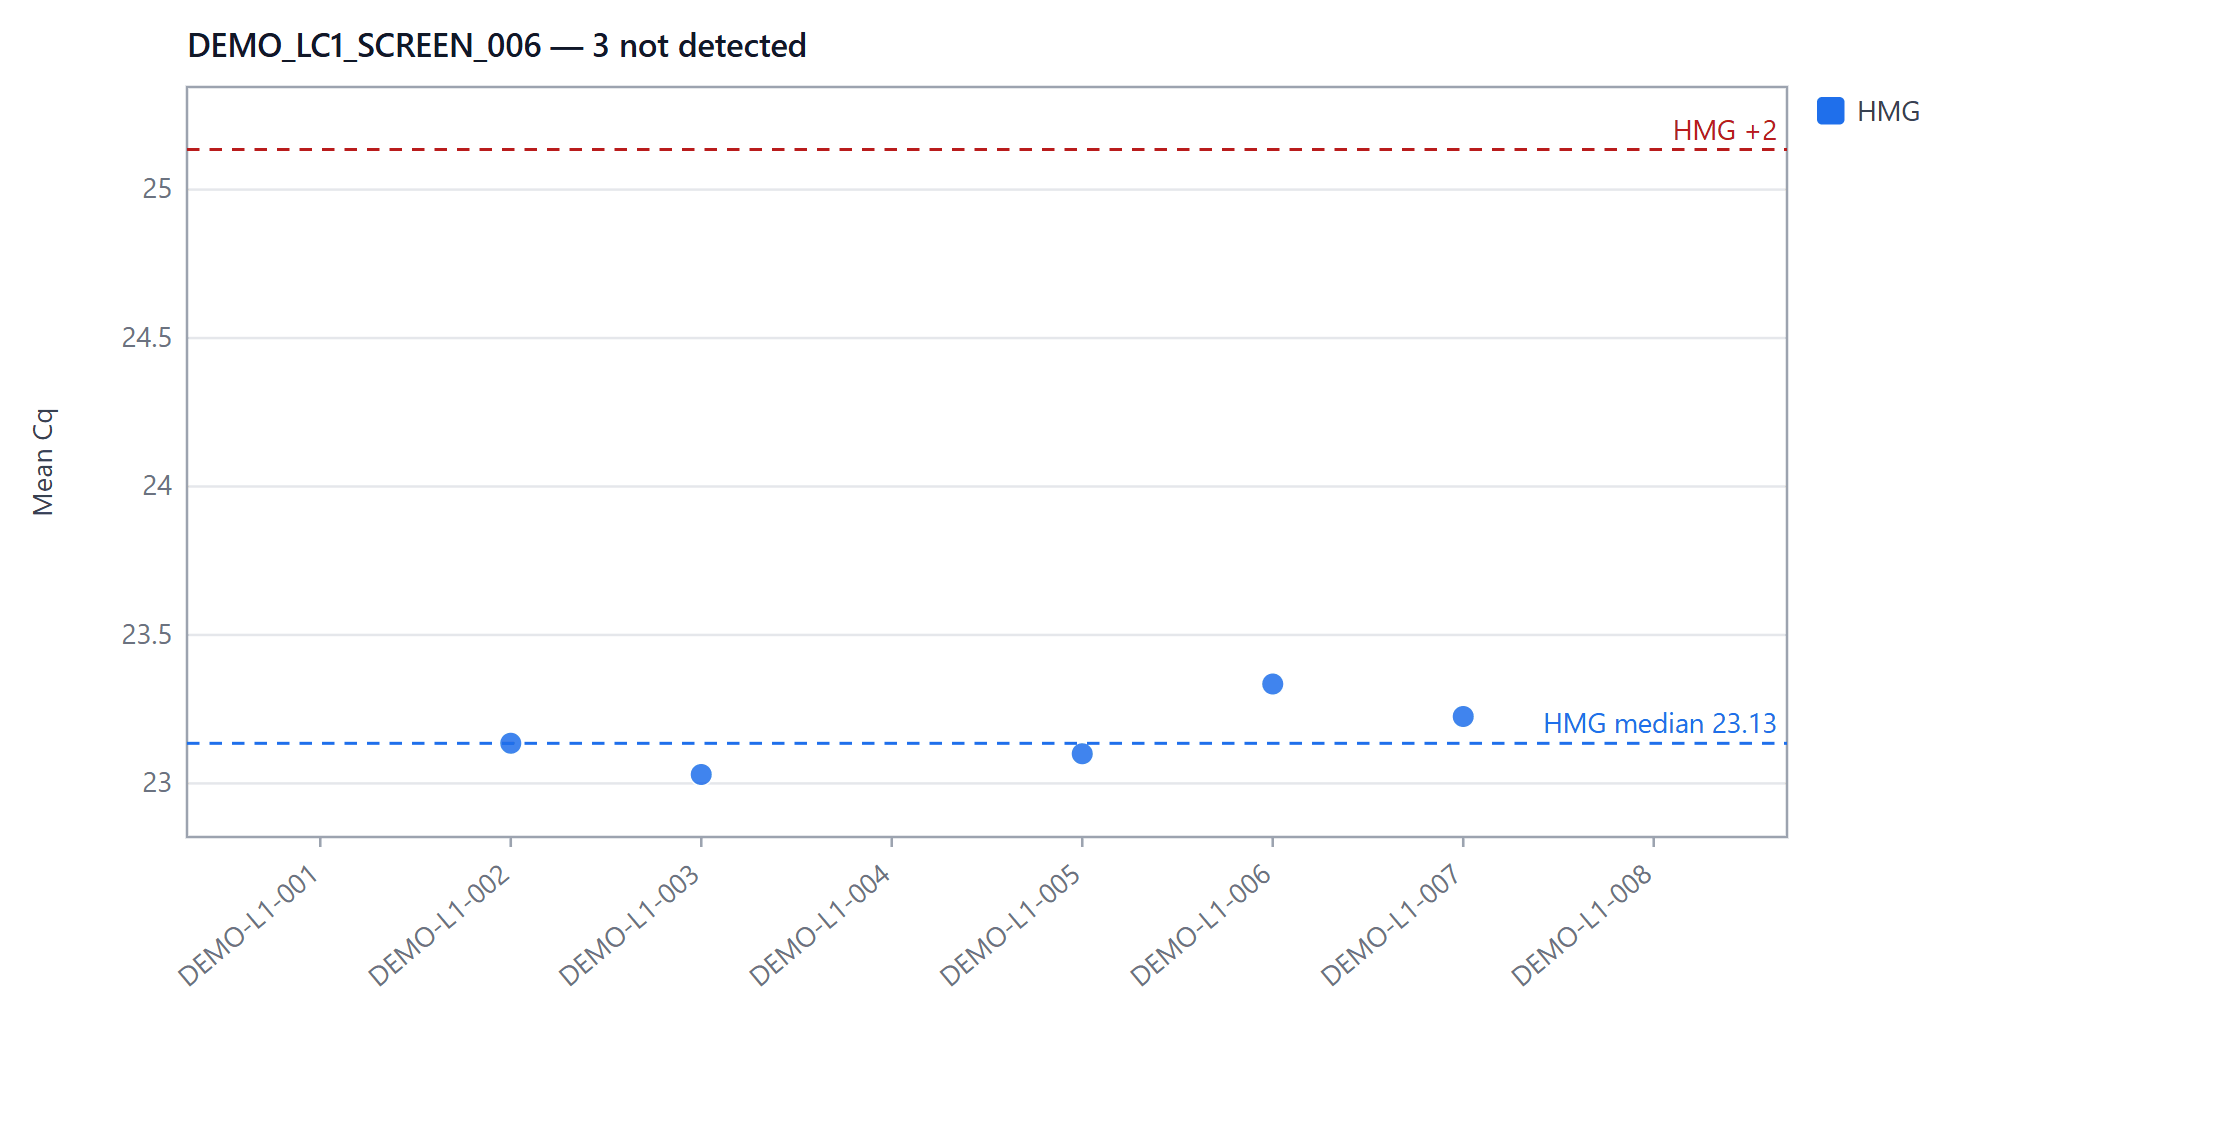
\includegraphics[width=\linewidth]{fig/g_LC_ic.png}\caption{\texttt{ic}: reference / IC Cq per sample}\end{subfigure}
\caption{\synthtag Replicate precision and reference-gene / internal-control graphs.}\label{fig:repsd_graphs}
\end{figure}
\fig[0.85]{g_QC_stdcurve.png}{\texttt{stdcurve} — standard curve of the synthetic dilution series with slope, R$^2$ and efficiency judged against the SOP (90--110\,\%, R$^2\ge0.98$, $\ge3$ logs).}{g_QC_stdcurve}
\fig[0.85]{g_QS_recalc.png}{\texttt{recalc} — stored Ct minus the Ct re-derived on the page from the stored $\Delta$Rn and threshold (.eds instrument). Points outside $\pm0.2$ would be flagged.}{g_QS_recalc}

\section{Graphs across all runs}
Cross-run graphs place the runs in date order; with more than 40 runs the axis shows dates instead of run names.

\par\medskip\noindent{\small\textbf{Listing}~\texttt{gRunDate()}\hfill\textcolor{gray}{HTML lines 5052--5052}}\par\nopagebreak
\lstinputlisting[style=vstyle,language=JavaScript,firstnumber=5052]{code/gRunDate.js}


\par\medskip\noindent{\small\textbf{Listing}~\texttt{gByDate()}\hfill\textcolor{gray}{HTML lines 5053--5053}}\par\nopagebreak
\lstinputlisting[style=vstyle,language=JavaScript,firstnumber=5053]{code/gByDate.js}


\par\medskip\noindent{\small\textbf{Listing}~\texttt{gRunTicks()}\hfill\textcolor{gray}{HTML lines 5054--5059}}\par\nopagebreak
\lstinputlisting[style=vstyle,language=JavaScript,firstnumber=5054]{code/gRunTicks.js}



\fig[0.85]{g_all_x_timeline.png}{\texttt{x\_timeline} — runs on a calendar (upper part): run (green), experiment created (blue), last change (red, joined by a dashed line).}{g_all_x_timeline}
\fig[0.9]{g_all_x_delay.png}{\texttt{x\_delay} — hours from run end to the last recorded change, log scale, SOP limit 72\,h. The planted 410\,h change of run 018 is red.}{g_all_x_delay}
\fig[0.8]{g_all_x_accept.png}{\texttt{x\_accept} — run acceptance grid: runs (rows) against the SOP criteria (columns), upper part.}{g_all_x_accept}
\fig[0.9]{g_all_x_outcomes.png}{\texttt{x\_outcomes} — stacked SOP outcomes per run.}{g_all_x_outcomes}
\fig[0.9]{g_all_x_control.png}{\texttt{x\_control} — descriptive control Cq across runs with the configured SOP range; pooled mean/SD lines were removed.}{g_all_x_control}
\fig[0.9]{g_all_x_signal.png}{\texttt{x\_signal} — median background (dashed) and end-point fluorescence (solid) per channel and run.}{g_all_x_signal}


